    Before discussing our previous work on this project, it is important to have
some background information on computer logic. There are primarily two forms of logic (Sequential and Combina-
tional). Traditional in electronic computers, sequential logic requires the use of memory elements, which are not available on quantum computers. However, for algorithms that do require extensive use of memory, we will create mixed signal
digital-quantum circuits, which can contain memory elements, while also making use of quantum compu-
tation. Combinational logic on the other hand does not require memory elements, and simply propagates
input values into output responses.


    \begin{wrapfigure}{R}{0.5\textwidth}
   \begin{center}
\begin{tabular}{|c|c||c|c|}
\hline
a&b&sum&carry-out \\
\hline 
0&0&0&0 \\
0&1&1&0 \\
1&0&1&0 \\
1&1&0&1 \\
\hline
\end{tabular}
  \end{center}
\end{wrapfigure}
One advantage to this project is that a tool which can handle the synthesis of quantum designs given a verilog specification has already been developed. Verilog is a computer-aided-circuit design description language, meaning it is used to specify the functionality of circuits before they are fabricated.  
As part of the project, this tool will be refined, and utilized to synthesize verilog descriptions of numerical methods into their equivalent quantum forms. 
We will then use an existing quantum simulator to evaluate the speedups that are experienced when using a quantum method for the solution. 
The tool was developed by Micah Thornton, and relies on existing software packages. 





The diagram below represents pictorially what the tool does. We start out with a single half-adder specified in purely combinational logic in Verilog. A half-adder is an electronic circuit that adds two bits together, the truth table for this circuit is given above.


By using the quantum synthesis tool we were able to extract the transfer matrix for this logical operation and convert it into a quantum circuit description. This is a very small example, but it illustrates the power of the tool, that performed this conversion automatically.
\begin{center}
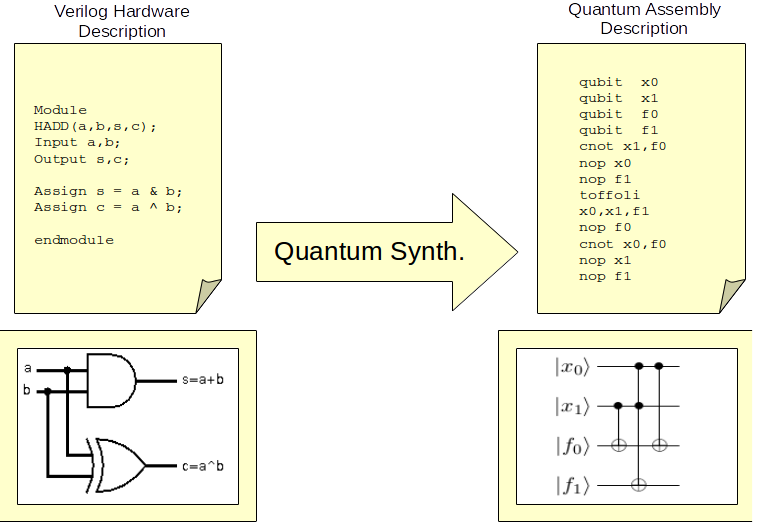
\includegraphics[scale=0.4]{QuantumSynthesis.png}
\end{center}

This quantum synthesis tool allows us to simply implement the numerical methods in combinational logic and then convert into a quantum assembly definition which can be simulated using any of the wealth of quantum logic simulators readily available online.